\subsection{实验目的}
理解遥感图像目标检测的概念,根据之前所完成的实验以及所学习的算法自主设计目标检测方法,完成遥感图像的目标检测。
\subsection{实验原理}
\subsubsection{目标检测的概念}
从大场景的遥感图像中检测出感兴趣的目标。例如舰船目标,车辆目标等。给出目标的位置信息,并在原始图像中标注出来检测出的目标,提供目标的切片图像,用于后续的目标识别。
\subsubsection{目标检测的一般流程}
\begin{figure}[H]
	\centering
	\begin{tikzpicture}[node distance=4cm]
	\node[process](original_rs_img){原始遥感图像};
	\node[process, right of=original_rs_img](binary_detection){二值检测结果图像};
	\node[process, right of=binary_detection](abstract_optional_objs){候选目标提取};
	\node[process,right of=abstract_optional_objs](remove_false_alert){虚警去除};
	
	\draw[->] (original_rs_img) -- (binary_detection);
	\draw[->] (binary_detection) -- (abstract_optional_objs);
	\draw[->] (abstract_optional_objs) -- (remove_false_alert);
	\end{tikzpicture}
\end{figure}
\subsubsection{二值检测结果}
通过设计目标检测算法,从原始的遥感图像得到一个输出图像,该图像与原始图像具有相同的大小,但是为一幅二值图像,其中值为1的点代表目标像素点,值为0的点代表非目标像素点。
\begin{description}
	\item[目标检测的本质] 寻找目标与周围背景的差异性,根据这个差异性寻找目标。
	\item[一种可能的思路] 判断每一个像素点与它周围的背景像素点的差异性,如果差异性足够大,则该像素点判定为属于目标。
\end{description}
\subsubsection{目标检测的滑窗模型}
\begin{figure}[H]
	\centering
	\begin{tikzpicture}
	\filldraw[fill=blue!30] (0, 0) rectangle ++(5, 5) node[right] {背景窗};
	\filldraw[fill=yellow] (.5, .5) rectangle ++(4, 4) node[pos=0.8] {警戒窗};
	\filldraw[fill=lightgray] (2.25, 1.75) rectangle ++(2, 1) node[pos=0.8]{目标大小};
	\filldraw[fill=red] (2.25, 2.25) rectangle ++(.5, .5) node[pos=0.8, above]{当前检测的像素点};
	\end{tikzpicture}
\end{figure}
\subsection{实验流程}
\begin{figure}[H]
	\centering
	\begin{tikzpicture}[node distance=1.5cm]
	\node[startstop](begin){开始};
	\node[io, below of=begin](read_img){读取待检测图片};
	\node[process, below of=read_img](loop_detection){循环滑窗检测};
	\node[process, below of=loop_detection](calculate_mean){计算背景窗像素点RGB均值};
	\node[process, below of=calculate_mean](calculate_std){计算背景窗像素点RGB方差};
	\node[decision,below of=calculate_std, node distance=5cm](judge_obj){判断检测像素点RGB值是否在$N\sigma$内};
	\node[process, below of=judge_obj, node distance=5cm](is_obj){在二值图上标记这个点};
	\node[process, right of=is_obj, node distance=5cm](not_obj){不做任何处理};
	\node[io, below of=is_obj](output_result){输出二值图};
	\node[startstop, below of=output_result](end){结束};
	
	\draw[->] (begin) -- (read_img);
	\draw[->] (read_img) -- (loop_detection);
	\draw[->] (loop_detection) -- (calculate_mean);
	\draw[->] (calculate_mean) -- (calculate_std);
	\draw[->] (calculate_std) -- (judge_obj);
	\draw[->] (judge_obj) -- (is_obj) node[pos=0.5, right] {是};
	\draw[->] (is_obj) -- (output_result);
	\draw[->] (output_result) -- (end);
	\draw[->] (judge_obj) -| (not_obj) node[pos=0.5, right] {否};
	\draw[->] (not_obj) |- (output_result);
	\end{tikzpicture}
\end{figure}
\subsection{实验程序}
\lstinputlisting[caption={ReadBridge47.m}]{"../Executable Script/Exp 7/ReadBridge47.m"}
\lstinputlisting[caption={ReadBridge48.m}]{"../Executable Script/Exp 7/ReadBridge48.m"}
\lstinputlisting[caption={ReadBridge50.m}]{"../Executable Script/Exp 7/ReadBridge50.m"}
\lstinputlisting[caption={WindowDetection.m}]{"../Function Library/WindowDetection.m"}
\subsection{实验结果和分析}
\begin{figure}[H]
	\centering
	\begin{minipage}{0.45\linewidth}
		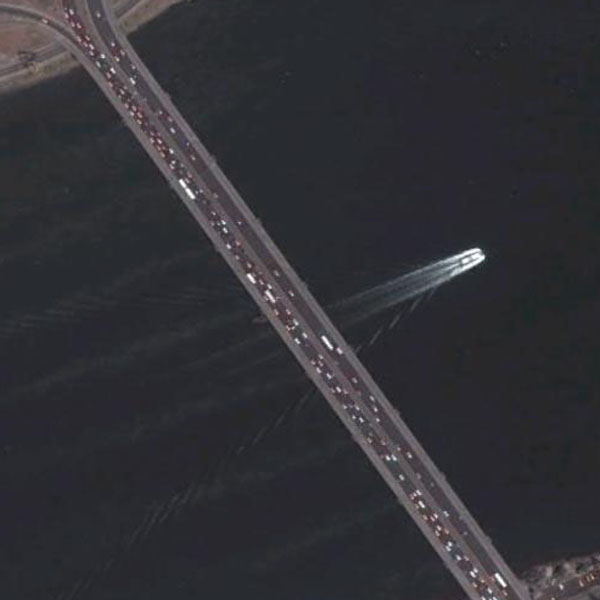
\includegraphics[width=\linewidth]{figure/bridge_47.jpg}
		\caption{bridge\_47原图}
	\end{minipage}
	\begin{minipage}{0.45\linewidth}
		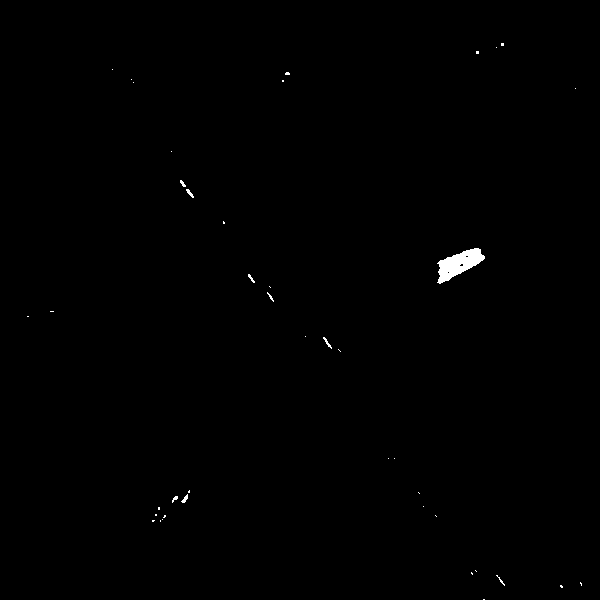
\includegraphics[width=\linewidth]{figure/bridge_47_detection.png}
		\caption{bridge\_47检测结果}
	\end{minipage}
\end{figure}
\begin{figure}[H]
	\centering
	\begin{minipage}{0.45\linewidth}
		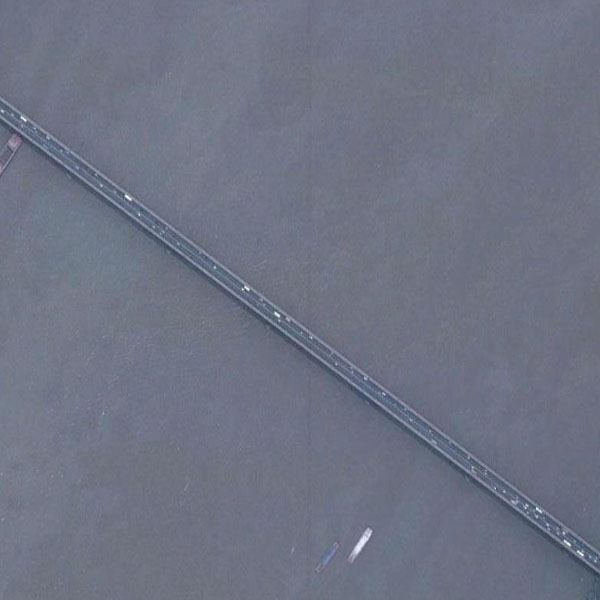
\includegraphics[width=\linewidth]{figure/bridge_48.jpg}
		\caption{bridge\_48原图}
	\end{minipage}
	\begin{minipage}{0.45\linewidth}
		
\includegraphics[width=\linewidth]{figure/bridge_48_detection.png}
		\caption{bridge\_48检测结果}
	\end{minipage}
\end{figure}
\begin{figure}[H]
	\centering
	\begin{minipage}{0.45\linewidth}
		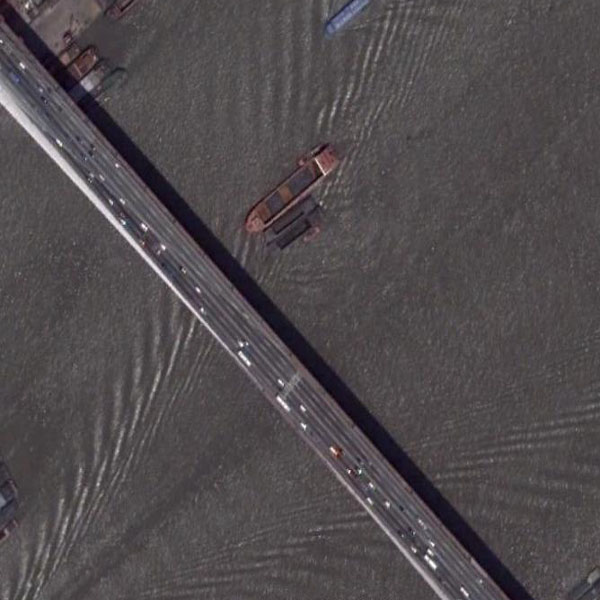
\includegraphics[width=\linewidth]{figure/bridge_50.jpg}
		\caption{bridge\_50原图}
	\end{minipage}
	\begin{minipage}{0.45\linewidth}
		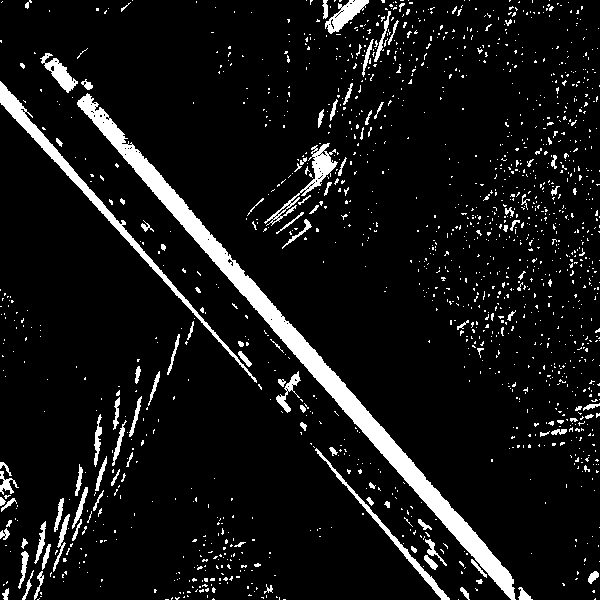
\includegraphics[width=\linewidth]{figure/bridge_50_detection.png}
		\caption{bridge\_50检测结果}
	\end{minipage}
\end{figure}

如上图所示是对三幅图的检测结果,其中检测结果中的白色区域是程序判定为目标点的位置,黑色区域是程序判定为不是目标区域的部分。可以看到对于bridge\_47和bridge\_48的检测结果比较理想,其中对真实目标的检测结果比较清晰,虚警目标极少。对bridge\_50的判定结果较差,虚警目标较多,对真实目标的判定不够清晰,对同一目标的检测不能形成连通区域。